

\section{Effect on an electric guitar}
In order to give an electrical guitar effect, all commently used effect needs to be analysed. This section aims is to give a overview of all frequently used guitar effect. These effect is: 

\begin{itemize}
 \item Equalizing
 \item Reverberation
 \item Overdrive
 \item Distortion
 \item Chorus
 \item Flanger
 \item Wah-Wah
\end{itemize}

To give an owerviwe how the effect influence the sound, all effect is descriped below

\newpage

\input{chapters/analysing/equalizing}\label{sec:equalizing} 
\section{Delay}
Delay is an audio effect which memorize the input signal for a customized time, and then release the signal without change the signal. The delayed signal can ether be played back multiple times witch make echo, or only delay the signal for the specified time. When the signal is delayed and played back multiple times, the delayed signal must be attenuated, unless the signal will keep moving in infinity time and depending on component tolerance, the delayed signal will be amplified or attenuated. If the delay is amplified the signal will start oscillate, so in analog delay unit the delayed signal needs to be attenuated to avoid oscillation. The \autoref{fig:delay_block} shows a block diagram over a simple delay, "echo" unit.


\begin{figure} [htbp]
 \centering
  \includegraphics[width=0.8\textwidth]{delay_block}
  \caption{The photo shows a block diagram on a delay unit}
  \label{fig:delay_block}
\end{figure}

The \autoref{fig:delay_block} shows a delay unit with feedback line, where the gain is adjusted. The feedback signal is attenuated and added to the delay line. This will continue until the signal is completely attenuated. This kind of delay give the echo effect, and this effect is the delay effect in guitar effect unit. The following \autoref{fig:delay_echo} shows the effect in time domain.

\begin{figure} [htbp]
 \centering
  \includegraphics[width=1\textwidth]{delay_echo}
  \caption{The photo shows a echo in time domain}
  \label{fig:delay_echo}
\end{figure}

http://www.hobby-hour.com/guitar/delay_effects.php\label{sec:delay} 
\subsection{Reverberation}
\gls{reverb} is an effect where the sound wave is reflected, and therefore the reflected waves haves another travelling time and amplitude to the listener than the initial sound directly from the source to the listener. This effect is a very frequently effect which happens each time sound can be reflected by walls, trees, table and other surfaces which reflect sound. The following \autoref{fig:reverb_reflect} shows the \gls{reverb} effect form one person, the sound source to another person, the listener \citep{reverb_expl}.

\begin{figure} [htbp]
 \centering
  \includegraphics[width=0.6\textwidth]{reverb_reflect}
  \caption{The photo shows a echo in time domain}
  \label{fig:reverb_reflect}
\end{figure}

The received reflected sound is actually a series of very fast echo, which is merged together with all other reflected- and the direct sound, so the effect is notice as a single effect, although that may be more than 100 echos. 
\gls{reverb} make a complex echo which bring depth to the guitar sound, and make the sound from the guitar more natural \citep{reverb_natural}

A simple block diagram is shown at \autoref{fig:reverb_block}.

\begin{figure} [htbp]
 \centering
\begin{picture}(0,0)%
\includegraphics{reverb.pdf}%
\end{picture}%
\setlength{\unitlength}{4144sp}%
\begingroup\makeatletter\ifx\SetFigFont\undefined%
\gdef\SetFigFont#1#2#3#4#5{%
  \reset@font\fontsize{#1}{#2pt}%
  \fontfamily{#3}\fontseries{#4}\fontshape{#5}%
  \selectfont}%
\fi\endgroup%
\begin{picture}(5787,3102)(886,-1603)
\put(5896,-286){$Output$}%
\put(4321,704){$Gain$}%
\put(2791,1334){Initial sound directly from the source}%
\put(901,1334){$Input$}%
\put(2791,434){$Delay$}%
\put(2791,-466){$Delay$}%
\put(2791,-1366){$Delay$}%
\put(4321,-241){$Gain$}%
\put(4321,-1141){$Gain$}%
\end{picture}%
  \caption{The photo shows a block diagram on a \gls{reverb} unit}
  \label{fig:reverb_block}
\end{figure}

The block diagram \autoref{fig:reverb_block} shows the direct sound way and only few delay block with individual gain, normally there will be many more delay lines. In the end, just before the Output line, all signals are added together.  \label{sec:reverberation} 
\section{Overdrive and Distortion} 

The distortion effects changes the sound of the played instrument by increasing the gain. It is commonly used in the with the electric guitar. The sound changes due to the clipping effect. \\
the clipping effect is way of changing the waveform when an amplifier is over driven; forcing it to deliver an output that is higher than its maximum capability. \\
The part of the waveform where the amplifier is asked to get a value higher than its maximum capacity gets the maximum value the amplifier can give. It means that all the parts of the waveform where the amplifier is pushed more than its capacity will have the same amplitude. The signal is then 'clipped'. An illustration of this effect is shown in \autoref{fig:clipping1}.\\

\begin{figure} [htbp]
  \includegraphics[width=0.7\textwidth]{clippingeffect.jpg}
  \caption{Photo showing the effect of clipping, a consequence of the overdrive or distortion effect.}
  \label{fig:clipping1}
\end{figure}


The consequences in the frequency domain are that the clipping effect creates more harmonics at high frequency than the signal without the clipping effect. \\

The clipping effect in signal processing happens when the amplitude is limited by a number and if during the processing the amplitude surpasses this limit, clipping happens because the value is then maxed to the maximum number that can be handled digitally. The maximum amplitude that can be handled is determined by the number of bits the system uses. The maximum number for a 16bit signed integers system is $\frac{2^{16}}{2} = 32768$ which means that if a value has an amplitude higher than this number the clipping effect occurs. \\

In any clipping technique, there is a creation of new harmonics. In the case of soft clipping, the new harmonics are multiples of the harmonics of the original tone. Valve Overdrive is a soft clipping technique for instance. In the case of hard clipping, they are not multiples which results to what is called intermodulation. Hard clipping usually happens when the harmonics of the original signal are not related by a multiple. Transistor overdrive is an example of hard clipping.\\
\label{sec:overdrive} 
\subsection{Chorus and Flanger Effect}

The chorus effect is obtained when a sound is delayed and then mixed with its original version. 
The chorus effect generator takes as an input a single audio signal and applies different delay values on it. Chorus effect can be applied using one delay. Each of the delayed signal are then mixed with original audio input. 
An \gls{lfo} (Low Frequency Oscillator) can be used to make the delay times vary. Different \gls{lfo}s can be used for each of the delay channels to make a richer sound mix and avoiding repetitive sound but it implies more computations. The same \gls{lfo} can be used for all the delay channels but not at the same cycle for each delay. \\

Different parameters can be changed to tune the chorus effect:\\
\begin{itemize}
\item \textbf{Delay time}: the time difference between the original sound and the delayed one.
\item \textbf{Chorus size}: the number of delayed sounds that will be mixed.
\item \textbf{Depth}: the amplitude of the of the modulation frequency.
\end{itemize}

The flanger effect is the same as the chorus effect but with shorter delay times.

A block diagram for  the chorus effect is shown in figure \autoref{fig:chorus_diag}.

\begin{figure} [htbp!]
	\centering
\begin{picture}(0,0)%
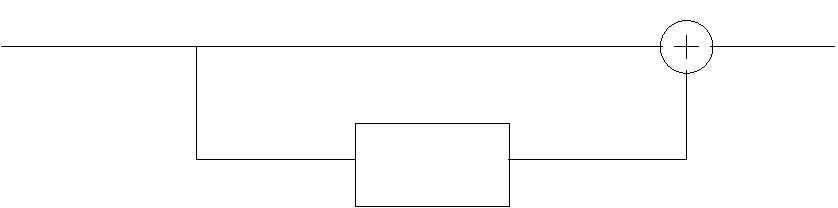
\includegraphics{chorus_diag.pdf}%
\end{picture}%
\setlength{\unitlength}{4144sp}%
%
\begingroup\makeatletter\ifx\SetFigFont\undefined%
\gdef\SetFigFont#1#2#3#4#5{%
  \reset@font\fontsize{#1}{#2pt}%
  \fontfamily{#3}\fontseries{#4}\fontshape{#5}%
  \selectfont}%
\fi\endgroup%
\begin{picture}(6327,1713)(3766,-2188)
\put(9406,-646){$Output$}%
\put(6706,-1186){$LFO$}%
\put(6436,-1906){$Delay$}%
\put(8101,-1636){$Gain$}%
\put(3781,-646){$Input$}%
\end{picture}%

\caption{Block Diagram of the chorus effect.}
\label{fig:chorus_diag}
\end{figure}


As it can be seen on the block diagram in figure \autoref{fig:chorus_diag}, a signal that hasn't been affected by any changes is added to the same one but with a delay. The addition is done just before the output. This represents the chorus effect.







\label{sec:chorus} 
\section{Wah-Wah}

The effect takes the original signal and mix it with the signal after passing through a bandpass filter. The bandpass filter is time varying, which means that it changes its position in the frequency spectrum. \\
Different parameters can be changed on the LFO to customize the effect:\\

\begin{itemize}
	\item \textbf{The LFO frequency}: it sets the speed at which the bandpass filter moves in the frequency spectrum.
	\item \textbf{LFO start phase}: Determine where should the bandpass filter start.
	\item \textbf{LFO depth} : the range of frequencies it should work on, high depth gives a bigger range and vice versa.
\end{itemize}

A block diagram of the effect is illustrated in.  
\label{sec:wah-wah} 
